\fancypage{\fbox}{}
\section{实验目的}
\begin{enumerate}
    \item 通过观测、分析RLC串联电路的相频和幅频特性,理解并学会具体应用特性。
    \item 进一步学习使用双踪示波器进行相位差的测量。
\end{enumerate}
\section{实验仪器}


正弦信号发生器、毫伏表、双踪数字示波器、自感器、电容器、交流电阻箱

\section{实验原理}
\subsection{RC串联电路的相频特性和幅频特性}
\begin{wrapfigure}[6]{r}{0.3\textwidth} %比如{r}{0.5\textwidth}
	\centering
	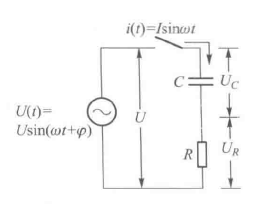
\includegraphics[height=3cm,width=5cm]{figure/1.png}
    \caption*{RC串联电路}
\end{wrapfigure}
在右图中,RC的总阻抗为$\tilde{Z}=R-j\dfrac{1}{\omega C}$,其模为$Z=|\tilde{Z}|=\sqrt{R^2+\left(\dfrac{1}{\omega C}\right)^2}$,其幅角为$\varphi=-\arctan \dfrac{1}{\omega CR}$,电容电阻两端的分压分别为
$$
U_R=\dfrac{U}{\sqrt{1+(\omega CR)^{-2}}},U_C=\dfrac{U}{\sqrt{1+(\omega CR)^{2}}}
$$
由以上公式可得该串联电路的如下特征
